
\documentclass{beamer}

% Common packages
\usepackage[utf8]{inputenc}
\usepackage[T1]{fontenc}
\usepackage{amsmath}
\usepackage{amsfonts}
\usepackage{amssymb}
\usepackage{graphicx}
\usepackage{tikz}
\usepackage{listings}
\usepackage{xcolor}
\usepackage{hyperref}

% TikZ libraries
\usetikzlibrary{positioning,arrows,shapes,calc}

% Code highlighting setup
\lstset{
    basicstyle=\ttfamily\footnotesize,
    keywordstyle=\color{blue},
    commentstyle=\color{green!60!black},
    stringstyle=\color{red},
    numbers=left,
    numberstyle=\tiny,
    breaklines=true,
    showstringspaces=false
}

% Title information
\title{Data Structures: Breadth-First Search (BFS)}
\author{Renn Gilbert}
\date{\today}

\begin{document}

% Title slide
\begin{frame}
\titlepage
\end{frame}

% Lesson overview
\begin{frame}
\frametitle{Lesson Overview}
\begin{itemize}
    \item Course context: Data Structures; Topic context: graphs and discrete math foundations.
    \item Objectives: understand BFS, implement it, analyze time and space, and apply it to shortest paths and connectivity.
    \item Prerequisites: graphs $(V,E)$, adjacency representations, and the queue data structure.
\end{itemize}
\end{frame}

% Graph definitions
\begin{frame}
\frametitle{Graphs: Definitions and Representations}
\begin{itemize}
    \item Graph $G=(V,E)$ with vertices $V$ and edges $E$; directed or undirected.
    \item Adjacency list: for each vertex, the list of neighbors. Space $\Theta(V+E)$.
    \item Adjacency matrix: $|V|\times|V|$ boolean matrix. Space $\Theta(V^2)$.
    \item BFS assumes efficient iteration over neighbors (e.g., adjacency lists).
\end{itemize}
\end{frame}

% BFS intuition
\begin{frame}
\frametitle{BFS: Intuition}
\begin{itemize}
    \item Explores vertices in nondecreasing distance from a source $s$.
    \item Uses a first-in first-out queue to manage the frontier.
    \item Produces a BFS tree and distances $\text{dist}[v]$ equal to the number of edges from $s$ to $v$ in unweighted graphs.
\end{itemize}
\end{frame}

% BFS pseudocode
\begin{frame}[fragile]
\frametitle{BFS: Pseudocode}
\begin{lstlisting}[language={},escapechar=!]
BFS(G, s):
    for each vertex v in V(G):
        visited[v] <- false
        dist[v] <- infinity
        parent[v] <- nil

    create an empty queue Q
    visited[s] <- true
    dist[s] <- 0
    enqueue(Q, s)

    while Q is not empty:
        u <- dequeue(Q)
        for each neighbor w in adj[u]:
            if not visited[w]:
                visited[w] <- true
                dist[w] <- dist[u] + 1
                parent[w] <- u
                enqueue(Q, w)
\end{lstlisting}
\end{frame}

% Why BFS works
\begin{frame}
\frametitle{Why BFS Works}
\begin{itemize}
    \item Layer invariant: when a vertex $u$ is dequeued, $\text{dist}[u]$ is the shortest-path length from $s$ to $u$.
    \item Queue discipline ensures vertices are processed in nondecreasing distance.
    \item Edges from a layer-$k$ vertex can only discover vertices in layer $k$ or $k+1$.
\end{itemize}
\end{frame}

% BFS example with TikZ
\begin{frame}
\frametitle{BFS Example on an Undirected Graph}
\centering
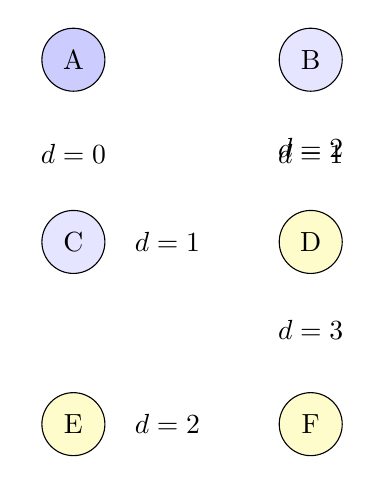
\begin{tikzpicture}[>=stealth, node distance=1.5cm, every node/.style={circle, draw, minimum size=8mm}]
\node[fill=blue!20] (A) {A};
\node[fill=blue!10, right=2.2cm of A] (B) {B};
\node[fill=blue!10, below=1.5cm of A] (C) {C};
\node[fill=yellow!20, right=2.2cm of C] (D) {D};
\node[fill=yellow!20, below=1.5cm of C] (E) {E};
\node[fill=yellow!20, right=2.2cm of E] (F) {F};

\path[thick]
(A) -- (B)
(A) -- (C)
(B) -- (D)
(C) -- (D)
(C) -- (E)
(D) -- (F)
(E) -- (F);

% Distances from A
\node[below=0.2cm of A, draw=none, fill=none] {$d=0$};
\node[below=0.2cm of B, draw=none, fill=none] {$d=1$};
\node[right=0.2cm of C, draw=none, fill=none] {$d=1$};
\node[above=0.2cm of D, draw=none, fill=none] {$d=2$};
\node[right=0.2cm of E, draw=none, fill=none] {$d=2$};
\node[above=0.2cm of F, draw=none, fill=none] {$d=3$};
\end{tikzpicture}

\small Colors indicate BFS layers from source A. Distances $d$ are shortest path lengths (in edges).
\end{frame}

% Complexity analysis
\begin{frame}
\frametitle{Complexity Analysis}
\begin{itemize}
    \item Time: $O(V+E)$ with adjacency lists. Each vertex is enqueued and dequeued once; each edge is inspected at most twice in undirected graphs (once in directed graphs).
    \item Space: $O(V)$ for \texttt{visited}, \texttt{dist}, \texttt{parent}, and the queue.
    \item With an adjacency matrix, time becomes $O(V^2)$ due to scanning rows for neighbors.
\end{itemize}
\end{frame}

% Path reconstruction
\begin{frame}[fragile]
\frametitle{Reconstructing a Shortest Path}
\begin{lstlisting}[language={},escapechar=!]
Path(s, t, parent):
    // assumes BFS has filled parent[]
    if t is nil:
        return empty list
    path <- empty list
    cur <- t
    while cur is not nil:
        prepend cur to path
        cur <- parent[cur]
    // path now lists vertices from s to t
    return path
\end{lstlisting}
\begin{itemize}
    \item Correctness: \texttt{parent[w]} is set when $w$ is first discovered via an edge on a shortest path.
    \item For unweighted graphs, BFS yields true shortest paths in number of edges.
\end{itemize}
\end{frame}

% Applications
\begin{frame}
\frametitle{Applications of BFS}
\begin{itemize}
    \item Shortest paths in unweighted graphs (e.g., level-order traversal in trees, simple routing).
    \item Connectivity: find all vertices reachable from a source; compute connected components by repeating BFS.
    \item Bipartite testing: 2-color the graph by parity of BFS layer; detect an odd cycle if an edge connects same-color vertices.
    \item Multi-source BFS: initialize the queue with multiple sources to compute distance to the nearest source.
\end{itemize}
\end{frame}

% Directed graphs
\begin{frame}
\frametitle{Directed Graphs and Edge Types}
\begin{itemize}
    \item BFS on directed graphs follows outgoing edges from each vertex.
    \item Traversal edges are tree edges; cross edges may connect layers but cannot reduce distances.
    \item Self-loops and parallel edges do not affect correctness when \texttt{visited} checks are used.
\end{itemize}
\end{frame}

% Implementation tips
\begin{frame}
\frametitle{Implementation Tips}
\begin{itemize}
    \item Use a queue from the standard library for efficiency.
    \item Initialize \texttt{dist} with a sentinel (for example, -1 or a large value) to mark unseen vertices.
    \item Choose data structures: vector of vectors or linked lists for adjacency; arrays or hash maps for \texttt{visited}, \texttt{dist}, and \texttt{parent}.
\end{itemize}
\end{frame}

% Edge cases
\begin{frame}
\frametitle{Edge Cases and Pitfalls}
\begin{itemize}
    \item Disconnected graphs: run BFS from multiple sources or repeat BFS to cover all vertices.
    \item Weighted graphs: BFS requires unit weights; use Dijkstra's algorithm for nonnegative weights.
    \item Early exit: to find a path from $s$ to $t$, you may stop when $t$ is dequeued; the \texttt{parent} array remains valid.
\end{itemize}
\end{frame}

% Practice
\begin{frame}
\frametitle{Practice}
\begin{itemize}
    \item Implement BFS on an undirected graph using an adjacency list. Report \texttt{dist} and \texttt{parent} arrays.
    \item Use BFS to test whether a given graph is bipartite and, if so, output the two color classes.
    \item Model a grid as a graph and use multi-source BFS to compute distance to the nearest exit.
\end{itemize}
\end{frame}

% Summary
\begin{frame}
\frametitle{Summary}
\begin{itemize}
    \item BFS explores vertices in increasing distance using a queue.
    \item It runs in $O(V+E)$ on adjacency lists and yields shortest paths in unweighted graphs.
    \item The \texttt{parent} array defines a BFS tree that supports path reconstruction and applications.
\end{itemize}
\end{frame}

% Further reading
\begin{frame}
\frametitle{Further Reading}
\begin{itemize}
    \item Cormen, Leiserson, Rivest, and Stein. Introduction to Algorithms, sections on BFS.
    \item Tarjan. Depth-first search and linear graph algorithms (for contrast with DFS).
    \item See also: \href{https://cp-algorithms.com/graph/breadth-first-search.html}{cp-algorithms: BFS}.
\end{itemize}
\end{frame}

\end{document}
